\section{Evolution de l'interface graphique}

Etant donné que nous appliquons la méthode SCRUM, le projet subit de nombreuses modifications au fur et à mesure que le projet avance. Procédant par itération, nous découvrons des contraintes avec l'interface que nous utilisons comme opportunités pour apporter des améliorations pour accueillir les fonctionnalités à ajouter. 

\begin{figure}[h!]
	\centering
	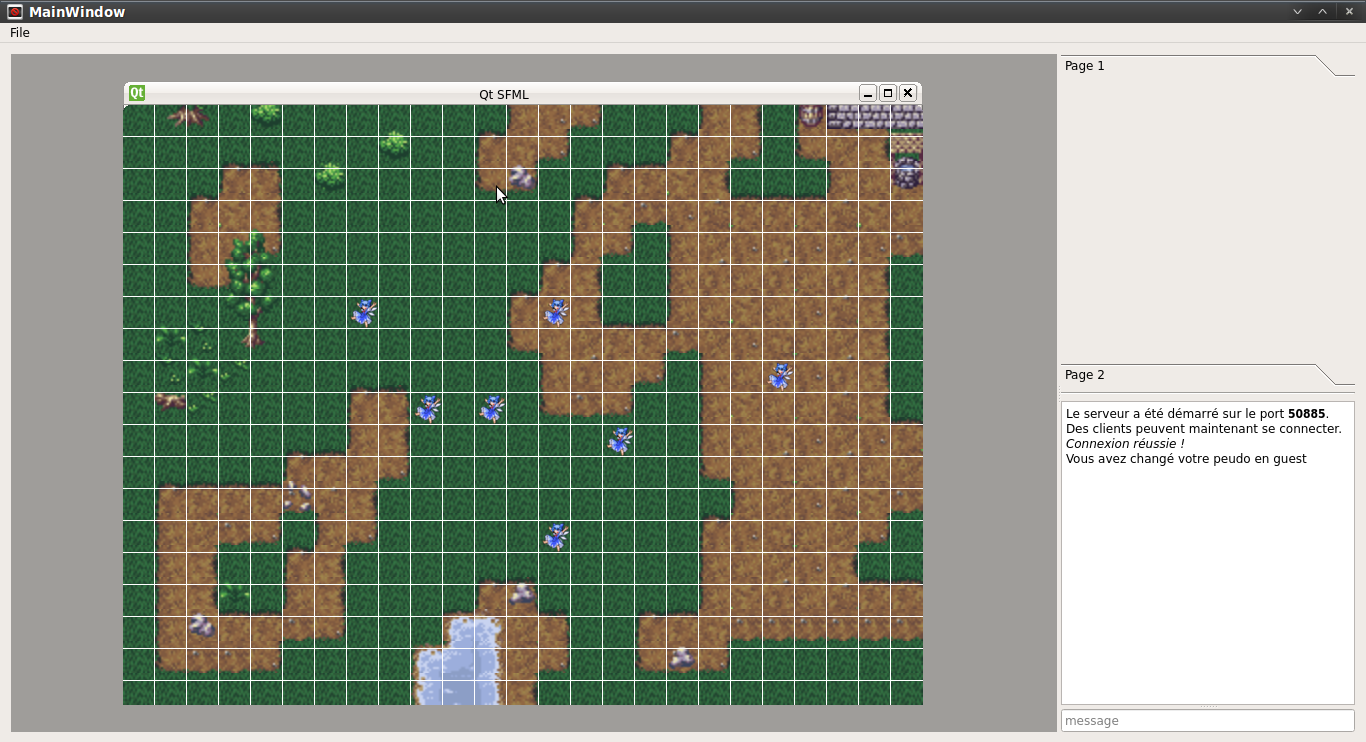
\includegraphics[width=0.8\textwidth]{img/gui_history/2014_05_07_screen.png}
	\caption{Interface du 7 Mai 2014}
\end{figure}

\begin{figure}[h!]
	\centering
	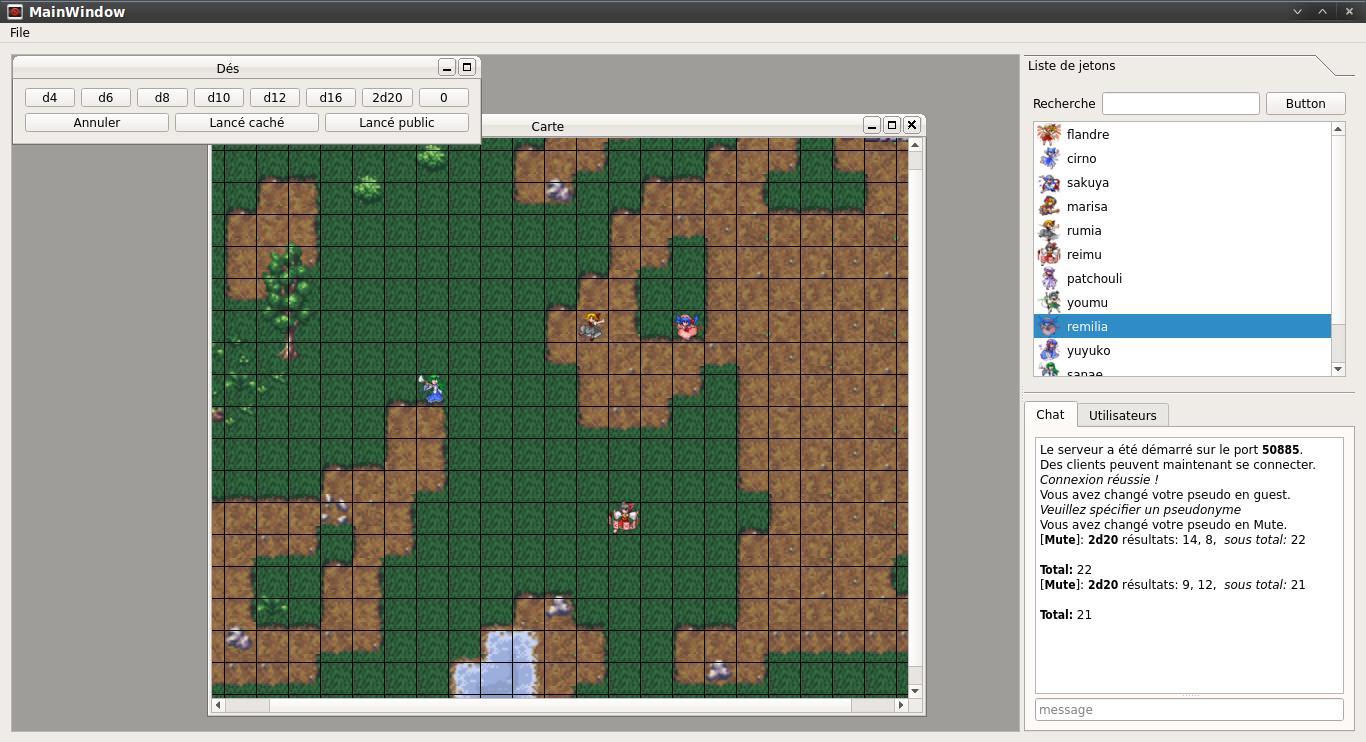
\includegraphics[width=0.8\textwidth]{img/gui_history/2014_05_21_screen.png}
	\caption{Interface du 21 Mai 2014 - Ajout des dés}
\end{figure}

\begin{figure}[h!]
	\centering
	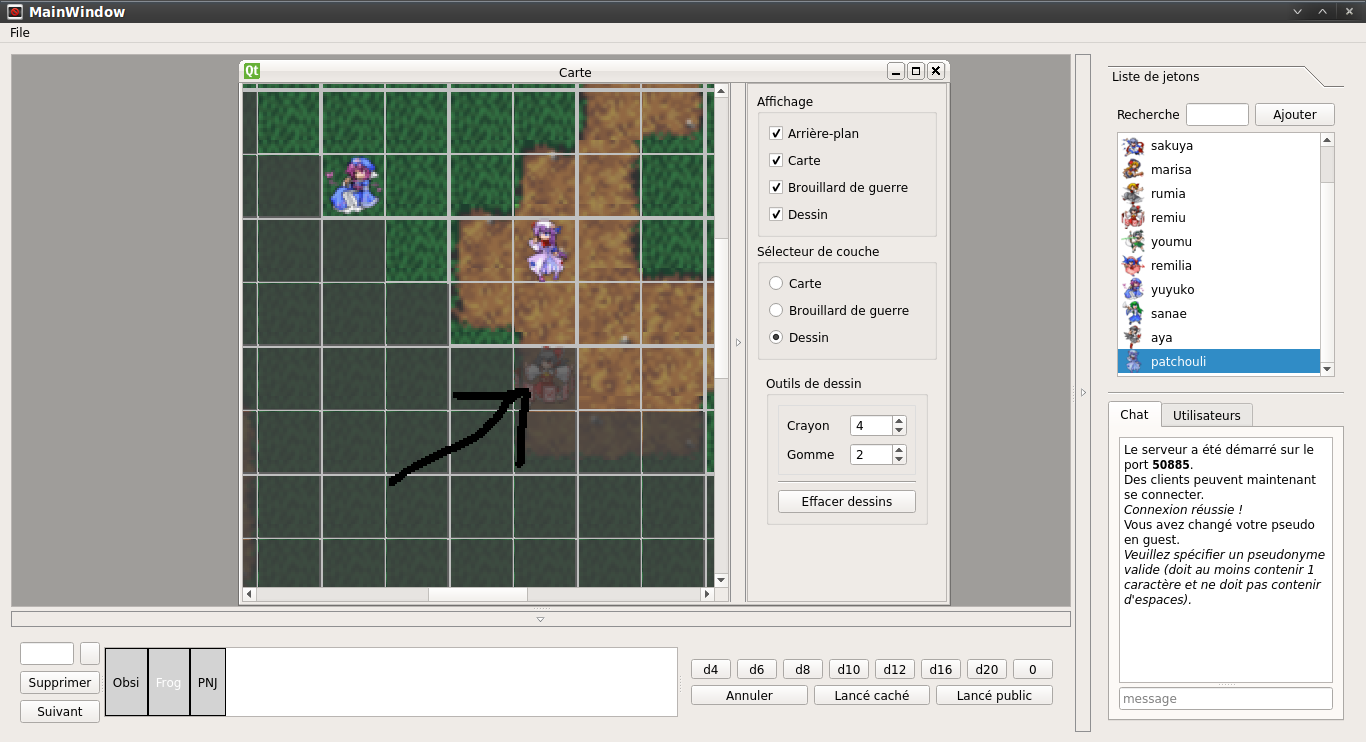
\includegraphics[width=0.8\textwidth]{img/gui_history/2014_05_30_screen.png}
	\caption{Interface du 30 Mai 2014 - Ajout du gestionnaire de tour + outils de carte}
\end{figure}

\begin{figure}[h!]
	\centering
	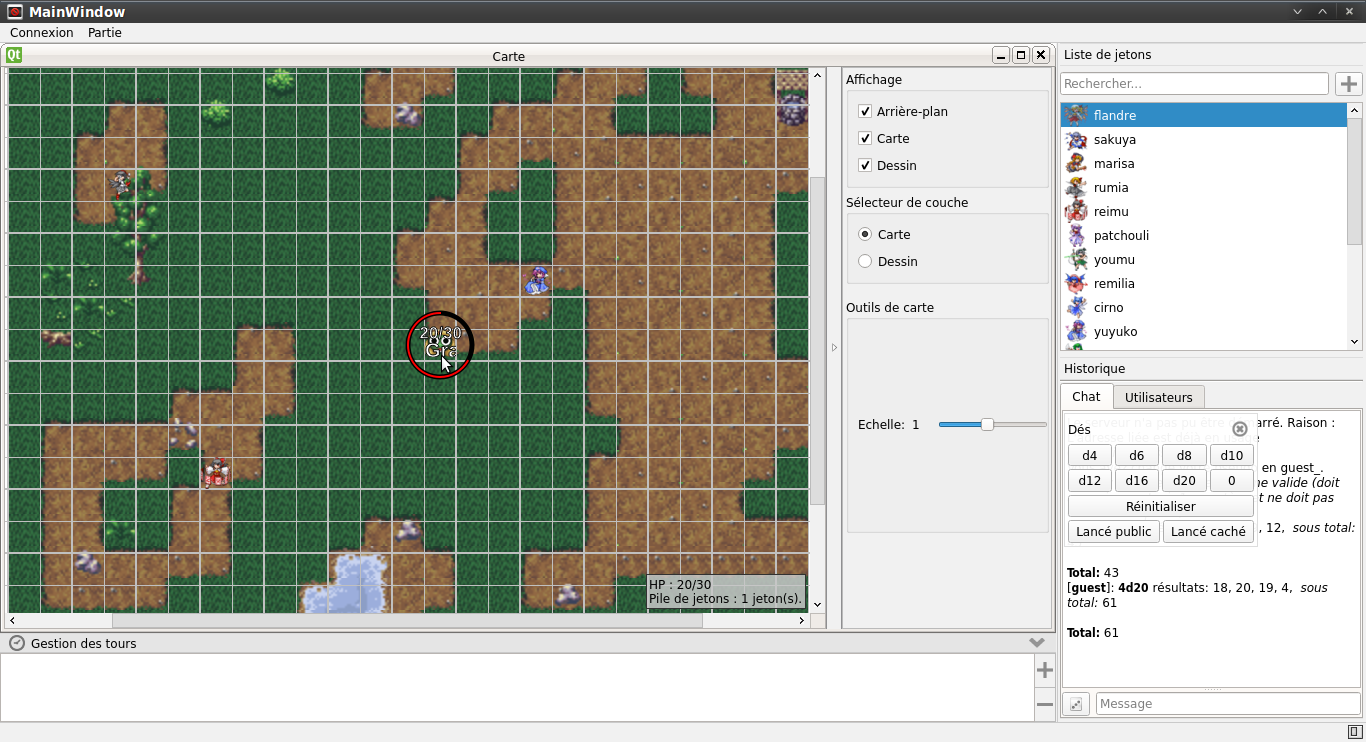
\includegraphics[width=0.8\textwidth]{img/gui_history/2014_06_18_screen.png}
	\caption{Interface du 18 Juin 2014 - Changement du style graphique}
\end{figure}

\section{Evolution technique} %outils
% \subsection
\section{SFML}

Au début de notre projet, nous avions pensé à utiliser une bibliothèque graphique spécialisée dans la réalisation de jeu, SFML (\textit{Simple and Fast Multimedia Library}).\\

Cette bibliothèque nous aurait permis de réaliser facilement des animations et toute sorte d'effet graphique. 
Cependant, en utilisant SFML, de mauvaises réactions ont été constatées, notamment au niveau de l'affichage de la fenetre SFML.
Après plusieurs difficultés à faire cohabiter Qt et SFML, nous avons, au bout de deux semaines, nous avons décidé de réaliser l'application exclusivement avec Qt. Pour cela, nous avons dû repenser entièrement le système de carte déjà réalisé avec SFML.
\subsection{Cpp2UML}

Afin d'avoir un rapide aperçu du projet ainsi qu'une vision globale des différentes classes réalisées et de leurs dépendance,
nous avons tenté de générer un diagramme \textit{UML} de notre projet.

Un diagramme \textit{UML} est une façon de représenter le code de manière graphique.
Ce diagramme est composé d'une bulle, représentant une classe dans laquelle y est inscrite la liste des membres et attributs de cette classe avec des information de portée (privé, publique ...).
Chacune de ces bulles sont ensuite reliées entre elles par différentes flèches symbolisant les relations entre deux classes. Il est possible d'obtenir les information filiales, d'utilisation ou encore de contenance.

\begin{figure}[h!]
	\centering
	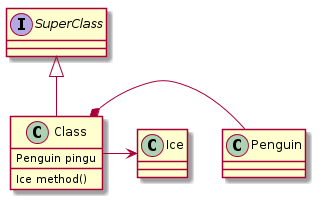
\includegraphics[width=0.6\textwidth]{img/uml_example.png}
	\caption{\textbf{Class} est une implementation d'une \textbf{SuperClass} qui utilise \textbf{Ice} et possède un \textbf{Penguin}, elle est composé d'un attribut \textit{pingu}, et d'une méthode \textit{surf}}
\end{figure}

Dans le cadre de notre projet, nous avons réalisé un script en \textit{Lua},
permettant de générer automatiquement ce genre de graphique par le biais d'un autre outil:
\href{http://plantuml.sourceforge.net/}{PlantUML}.

Ce script annalyse les en-têtes de nos sources afin d'écrire un autre fichier de description compréhensible par PlantUML. Une fois ceci fait,  plantUML, en utilisant graphviz, crée une image de notre diagramme UML.
